% Lecture notes with a wide outer margin for side notes.
% Edit the course details below; the page design lives in notes-style.tex.
% Each lecture starts with \lecture{number}{title}{date}.
\documentclass[11pt]{article}

\newcommand{\CourseCode}{MATH 2410}
\newcommand{\CourseName}{Fourier Analysis and PDEs}
\newcommand{\CourseTerm}{Fourier Analysis and PDEs \enspace\textperiodcentered\enspace Autumn 2026 \enspace\textperiodcentered\enspace Dr.\ Mira Okafor}

% Page design for the lecture notes. main.tex holds the content; change the
% course details there and the colours in the "Colour" block below.

% --- Type: XCharter text with matching math, Lato for display --------------
\usepackage[T1]{fontenc}
\usepackage[osf]{XCharter}          % old-style figures sit well in running text
\usepackage{amsmath,amssymb}
\usepackage[xcharter,vvarbb]{newtxmath}
\usepackage[defaultsans,lining,tabular,scale=0.92]{lato}
\usepackage[scaled=0.9]{zi4}        % Inconsolata for code
\usepackage[protrusion=true,expansion=true,tracking=true]{microtype}
\linespread{1.1}

% --- Page: a 118 mm measure with a 48 mm outer margin for notes ------------
\usepackage[a4paper,left=24mm,textwidth=118mm,marginparsep=7mm,
  marginparwidth=48mm,top=30mm,bottom=28mm,headsep=9mm,footskip=12mm,
  headheight=14pt]{geometry}
\setlength{\parindent}{1.2em}
\setlength{\parskip}{0pt}
\frenchspacing
\clubpenalty=10000
\widowpenalty=10000
\raggedbottom

% --- Colour: the accent and the four box tints ------------------------------
\usepackage{xcolor}
\definecolor{accent}{HTML}{0B5F5C}  % deep teal: headings, labels, key ideas
\definecolor{defcol}{HTML}{0B5F5C}  % definitions share the accent
\definecolor{thmcol}{HTML}{3D5A86}  % theorems: slate blue
\definecolor{excol}{HTML}{A8742B}   % examples: ochre
\definecolor{exercol}{HTML}{85506B} % exercises: muted plum
\colorlet{muted}{black!55}
\colorlet{hairline}{black!20}

% --- Small labels: tracked capitals in Lato ---------------------------------
\newcommand{\caps}[1]{{\sffamily\textls[120]{\MakeUppercase{#1}}}}
\newcommand{\latolight}{\sffamily\fontseries{l}\selectfont}
\newcommand{\latothin}{\sffamily\fontseries{el}\selectfont}
\newcommand{\latosemi}{\sffamily\fontseries{sb}\selectfont}

% --- Margin notes -----------------------------------------------------------
% marginnote works inside boxes and floats, where \marginpar does not.
\usepackage{marginnote}
\renewcommand*{\raggedrightmarginnote}{\raggedright}
\newcommand{\notefont}{\footnotesize\linespread{1.05}\selectfont\color{black!75}}
\newcounter{sidenote}
\newcommand{\sidenote}[2][0pt]{%
  \refstepcounter{sidenote}%
  \textsuperscript{\sffamily\color{accent}\thesidenote}%
  \marginnote{\notefont\llap{\textsuperscript{\sffamily\color{accent}\thesidenote}\,}#2}[#1]}
\newcommand{\margintext}[2][0pt]{\marginnote{\notefont #2}[#1]}

% --- Lecture openers --------------------------------------------------------
% \lecture{number}{title}{date} starts a page with the number set large in
% the margin and the title beside it, then resets section numbering.
\newcounter{lecture}
\newcommand{\currentlecture}{}
\newlength{\fullwidth}
\setlength{\fullwidth}{\dimexpr\textwidth+\marginparsep+\marginparwidth\relax}
\newcommand{\lecture}[3]{%
  \clearpage
  \setcounter{lecture}{#1}\setcounter{section}{0}%
  \gdef\currentlecture{Lecture #1\enspace\textperiodcentered\enspace #2}%
  \thispagestyle{opener}%
  \noindent
  \begin{minipage}[b]{\textwidth}
    {\color{accent}\footnotesize\caps{Lecture #1}}\par\vspace{3mm}
    {\latolight\fontsize{27}{31}\selectfont\raggedright #2\par}
  \end{minipage}%
  \rlap{\hspace{\marginparsep}%
  \begin{minipage}[b]{\marginparwidth}
    \raggedleft
    {\latothin\color{accent}\fontsize{76}{70}\selectfont #1\par}
    \vspace{1mm}
    {\footnotesize\color{muted}\caps{#3}}
  \end{minipage}}\par\vspace{4mm}
  \noindent\rlap{\color{accent}\rule{\fullwidth}{0.6pt}}%
  \par\vspace{9mm}}

% --- Headings ---------------------------------------------------------------
\usepackage{titlesec}
\renewcommand{\thesection}{\thelecture.\arabic{section}}
\titleformat{\section}
  {\sffamily\latosemi\large}
  {\color{accent}\thesection}{0.8em}{}
\titlespacing*{\section}{0pt}{2.2\baselineskip plus 4pt minus 2pt}
  {0.6\baselineskip}
\titleformat{\subsection}[runin]
  {\sffamily\latosemi\normalsize}{}{0pt}{}
\titlespacing*{\subsection}{0pt}{1.1\baselineskip plus 2pt minus 2pt}{0.6em}

% --- Running header: course code over the full width ------------------------
\usepackage{fancyhdr}
\pagestyle{fancy}
\fancyhf{}
\fancyhfoffset[R]{\dimexpr\marginparsep+\marginparwidth\relax}
\renewcommand{\headrulewidth}{0pt}
\fancyhead[L]{\footnotesize{\color{accent}\caps{\CourseCode}}\enspace
  {\color{hairline}|}\enspace{\sffamily\color{muted}\CourseName}}
\fancyhead[R]{\footnotesize\sffamily\color{muted}\currentlecture
  \hspace{1.4em}{\color{black}\thepage}}
\fancypagestyle{opener}{\fancyhf{}%
  \fancyhead[L]{\footnotesize{\color{accent}\caps{\CourseCode}}\enspace
    {\color{hairline}|}\enspace{\sffamily\color{muted}\CourseTerm}}%
  \fancyhead[R]{\footnotesize\sffamily\thepage}}

% --- Boxes: soft tint with a thin left bar, no frame ------------------------
\usepackage[most]{tcolorbox}
\tcbset{
  notebox/.style={enhanced,breakable,sharp corners,boxrule=0pt,frame hidden,
    colback=#1!6,borderline west={1.4pt}{0pt}{#1},
    left=4mm,right=4mm,top=2.6mm,bottom=2.6mm,
    before skip=\baselineskip,after skip=\baselineskip,
    fonttitle=\sffamily\footnotesize,coltitle=#1,
    detach title,before upper={\tcbtitle\enspace}},
  notetitle/.style={separator sign none,description delimiters none,
    description font=\upshape\sffamily\latosemi\small\color{black!80},
    terminator sign={\enspace}}}
\newcommand{\boxlabel}[1]{{\upshape\latosemi\caps{#1}}}
\newtcbtheorem[number within=lecture]{definition}{\boxlabel{Definition}}
  {notebox=defcol,notetitle}{def}
\newtcbtheorem[use counter from=definition]{theorem}{\boxlabel{Theorem}}
  {notebox=thmcol,notetitle,unbreakable,fontupper=\itshape}{thm}
\newtcbtheorem[use counter from=definition]{lemma}{\boxlabel{Lemma}}
  {notebox=thmcol,notetitle,unbreakable,fontupper=\itshape}{lem}
\newtcbtheorem[use counter from=definition]{example}{\boxlabel{Example}}
  {notebox=excol,notetitle}{ex}
\newtcbtheorem[use counter from=definition]{exercise}{\boxlabel{Exercise}}
  {notebox=exercol,notetitle}{exer}

% Worked solutions sit inside example boxes and end with a small teal square.
\newcommand{\qedmark}{{\color{accent}\rule{0.5em}{0.5em}}}
\newenvironment{solution}
  {\par\smallskip\noindent{\sffamily\latosemi\small\color{excol}Solution.}\enspace}
  {\hfill\qedmark\par}
\newenvironment{proof}
  {\par\smallskip\noindent{\sffamily\latosemi\small\color{thmcol}Proof.}\enspace}
  {\hfill\qedmark\par\smallskip}

% "Key idea": hairlines above and below, label set in the margin.
\newenvironment{keyidea}
  {\par\vspace{0.8\baselineskip}\noindent{\color{accent}\rule{\textwidth}{0.5pt}}%
   \par\nobreak\vspace{0.1\baselineskip}\noindent
   \marginnote{\footnotesize\color{accent}\latosemi\caps{Key idea}}[0.15\baselineskip]%
   \begin{minipage}[t]{\textwidth}\itshape\color{black!88}}
  {\end{minipage}\par\vspace{0.55\baselineskip}\noindent
   {\color{accent}\rule{\textwidth}{0.5pt}}\par\vspace{0.8\baselineskip}}

% --- Figures with captions in the margin ------------------------------------
\usepackage{pgfplots}
\pgfplotsset{compat=1.18}
\usepackage[font={footnotesize},labelfont={sf,color=accent},labelsep=quad,
  justification=raggedright,singlelinecheck=false]{caption}
\DeclareCaptionLabelFormat{lecture}{\caps{#1 #2}}
\captionsetup{labelformat=lecture}
\renewcommand{\thefigure}{\thelecture.\arabic{figure}}
\renewcommand{\thetable}{\thelecture.\arabic{table}}
% \sidecaption{body}{caption}: body in the text column, caption beside it.
\newcommand{\sidecaption}[2]{%
  \noindent\makebox[\textwidth][l]{%
    \begin{minipage}[b]{\textwidth}\centering #1\end{minipage}%
    \hspace{\marginparsep}%
    \begin{minipage}[b]{\marginparwidth}#2\end{minipage}}}

% --- Tables -----------------------------------------------------------------
\usepackage{booktabs,array}
\setlength{\heavyrulewidth}{0.6pt}
\setlength{\lightrulewidth}{0.3pt}
\renewcommand{\arraystretch}{1.3}

% --- Code -------------------------------------------------------------------
\usepackage{listings}
\lstset{basicstyle=\ttfamily\small,columns=fullflexible,keepspaces,
  keywordstyle=\color{accent}\bfseries,commentstyle=\color{muted},
  stringstyle=\color{excol},numbers=left,numberstyle=\tiny\sffamily\color{muted},
  numbersep=8pt,xleftmargin=5mm,framexleftmargin=5mm,frame=l,
  framerule=1.4pt,rulecolor=\color{accent!45},backgroundcolor=\color{black!3},
  framesep=3mm,aboveskip=\baselineskip,belowskip=0.6\baselineskip,
  showstringspaces=false,upquote=true}

% --- Lists and links --------------------------------------------------------
\usepackage{enumitem}
\setlist{itemsep=0.15\baselineskip,topsep=0.35\baselineskip,leftmargin=1.5em}
\setlist[enumerate]{label={\sffamily\small\color{accent}(\alph*)}}
\usepackage[hidelinks,pdfusetitle]{hyperref}


\hypersetup{pdftitle={MATH 2410 Lecture Notes},pdfauthor={Mira Okafor}}

\begin{document}

% ============================================================================
\lecture{3}{Fourier series}{Tuesday 6 October}

Last week we separated variables in the heat equation on a ring and found
solutions of the form $e^{-n^2 t}\cos nx$ and $e^{-n^2 t}\sin nx$. Any finite
sum of these is again a solution, so the obvious question is whether
\emph{every} initial temperature profile can be written as such a sum. Fourier
claimed in 1807 that it can, provided the sum is allowed to be
infinite.\sidenote{The claim met resistance from Lagrange, who doubted that a
discontinuous function could be a sum of smooth ones. Both were partly right;
see \S\ref{sec:gibbs}.} Today we make that claim precise for $2\pi$-periodic
functions and compute our first series.

\section{Periodic functions and an inner product}

A function $f\colon\mathbb{R}\to\mathbb{R}$ is \emph{$2\pi$-periodic} if
$f(x+2\pi)=f(x)$ for all $x$. Such a function is determined by its values on
any interval of length $2\pi$; we use $[-\pi,\pi)$ throughout. Geometry enters
through the following pairing, which behaves like a dot product with infinitely
many coordinates.

\begin{definition}{Inner product}{inner}
For integrable $2\pi$-periodic functions $f$ and $g$, set
\[
  \langle f,g\rangle = \frac{1}{\pi}\int_{-\pi}^{\pi} f(x)\,g(x)\,dx,
  \qquad \|f\| = \langle f,f\rangle^{1/2}.
\]
We call $f$ and $g$ \emph{orthogonal} when $\langle f,g\rangle=0$.
\end{definition}

The factor $1/\pi$ is a convention\margintext[-1.5\baselineskip]{Some texts use
$\tfrac{1}{2\pi}$ instead; the coefficient formulas then change by a factor of
two. Check which convention a source uses before copying a result.} chosen so
that $\cos nx$ and $\sin nx$ have norm one. The next lemma is the whole reason
the trigonometric functions are a good coordinate system.

\begin{lemma}{Orthogonality}{orth}
For integers $m,n\ge 1$,
\[
  \langle \cos mx, \cos nx\rangle = \langle \sin mx, \sin nx\rangle
  = \delta_{mn},
  \qquad
  \langle \cos mx, \sin nx\rangle = 0,
\]
and $\langle 1, 1\rangle = 2$, while $1$ is orthogonal to every $\cos nx$ and
$\sin nx$.
\end{lemma}

\begin{proof}
Use the product formula
$2\cos mx\cos nx = \cos(m-n)x + \cos(m+n)x$. The integral of $\cos kx$ over a
full period vanishes unless $k=0$, which happens only for the first term when
$m=n$. The other two cases follow in the same way from the corresponding
product formulas.
\end{proof}

\section{Fourier coefficients}

Suppose for a moment that $f$ really is a sum
$\tfrac{a_0}{2}+\sum_{n\ge1}(a_n\cos nx + b_n\sin nx)$ and that we may
integrate term by term. Taking the inner product with $\cos mx$ kills every
term except one, by Lemma~\ref{lem:orth}. This forces the coefficients and motivates
the definition.

\begin{definition}{Fourier series}{fs}
The \emph{Fourier coefficients} of an integrable $2\pi$-periodic $f$ are
\[
  a_n = \langle f, \cos nx\rangle, \qquad b_n = \langle f, \sin nx\rangle,
  \qquad n \ge 0,
\]
and its \emph{Fourier series} is the formal sum
\begin{equation}\label{eq:fs}
  f(x) \sim \frac{a_0}{2} + \sum_{n=1}^{\infty}\bigl(a_n\cos nx + b_n\sin nx\bigr).
\end{equation}
The $N$th \emph{partial sum} $S_N f$ stops the sum at $n=N$.
\end{definition}

The symbol $\sim$ is deliberate: nothing yet says the series converges, let
alone to $f$.\sidenote{Lecture~4 answers both questions for piecewise smooth
functions.} Two shortcuts save most of the work in practice. If $f$ is even,
every $b_n$ vanishes; if $f$ is odd, every $a_n$ vanishes.

\begin{example}{Square wave}{square}
Let $f(x)=\operatorname{sgn}(x)$ on $(-\pi,\pi)$, extended periodically.
Compute its Fourier series.
\begin{solution}
The function is odd, so $a_n=0$ for all $n$. For the sine coefficients,
\[
  b_n = \frac{2}{\pi}\int_0^{\pi}\sin nx\,dx
      = \frac{2}{\pi}\cdot\frac{1-\cos n\pi}{n}
      = \begin{cases} \dfrac{4}{\pi n}, & n \text{ odd},\\[4pt]
                      0, & n \text{ even}.\end{cases}
\]
Hence
$\operatorname{sgn}(x) \sim \frac{4}{\pi}\bigl(\sin x + \tfrac13\sin 3x
+ \tfrac15\sin 5x + \cdots\bigr)$.
\end{solution}
\end{example}

The coefficients decay only like $1/n$, which is slow. That is typical of a
function with a jump, and Figure~\ref{fig:square} shows what it costs.

\begin{figure}[t]
\sidecaption{%
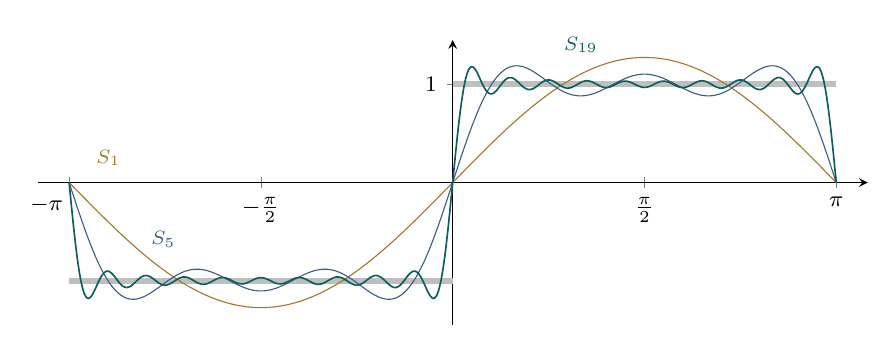
\begin{tikzpicture}
\begin{axis}[width=\textwidth,height=52mm,
  axis lines=middle,xmin=-3.4,xmax=3.4,ymin=-1.45,ymax=1.45,
  xtick={-1.5708,1.5708,3.1416},
  xticklabels={$-\frac{\pi}{2}$,$\frac{\pi}{2}$,$\pi$},
  % The curves start at -pi and fall below the axis, so its label sits to the left.
  extra x ticks={-3.1416},extra x tick labels={$-\pi$},
  extra x tick style={xticklabel style={anchor=north east,xshift=-1pt}},
  ytick={1},tick label style={font=\footnotesize},
  xticklabel style={fill=white,inner sep=1pt,yshift=-2pt},
  every axis plot/.append style={samples=400,smooth,domain=-3.1416:3.1416},
  clip=false]
\addplot[black!25,line width=2.2pt,domain=-3.1416:-0.001] {-1};
\addplot[black!25,line width=2.2pt,domain=0.001:3.1416] {1};
\addplot[excol,thin] {4/pi*sin(deg(x))};
\addplot[thmcol,thin] {4/pi*(sin(deg(x))+sin(deg(3*x))/3+sin(deg(5*x))/5)};
\addplot[accent,semithick] {4/pi*(sin(deg(x))+sin(deg(3*x))/3+sin(deg(5*x))/5
  +sin(deg(7*x))/7+sin(deg(9*x))/9+sin(deg(11*x))/11+sin(deg(13*x))/13
  +sin(deg(15*x))/15+sin(deg(17*x))/17+sin(deg(19*x))/19)};
\node[font=\scriptsize\sffamily,excol,anchor=west] at (axis cs:-3.0,0.25) {$S_1$};
\node[font=\scriptsize\sffamily,thmcol,anchor=west] at (axis cs:-2.55,-0.58) {$S_5$};
\node[font=\scriptsize\sffamily,accent,anchor=south] at (axis cs:1.05,1.22) {$S_{19}$};
\end{axis}
\end{tikzpicture}}{%
\caption{Partial sums of the square-wave series. Away from the jump they
settle down; next to it $S_5$ and $S_{19}$ overshoot by about 9\% of the jump.}
\label{fig:square}}
\end{figure}

\section{The Gibbs phenomenon}\label{sec:gibbs}

Look closely at the peaks next to $x=0$ in Figure~\ref{fig:square}. As $N$ grows the
overshoot moves closer to the jump but does not shrink. One can show that
\[
  \lim_{N\to\infty}\max_{x} S_N f(x) = \frac{2}{\pi}\int_0^{\pi}\frac{\sin t}{t}\,dt
  \approx 1.1790,
\]
an overshoot of roughly 9\% of the total jump of $2$.\sidenote[-2\baselineskip]{Named after
J.\,W.\ Gibbs, who described it in 1899, although Wilbraham had found it fifty
years earlier.}

\begin{keyidea}
Smoothness of $f$ and decay of its Fourier coefficients are two views of the
same thing. A jump gives coefficients of size $1/n$ and a persistent
overshoot; each extra continuous derivative buys one more power of $1/n$.
\end{keyidea}

\subsection{Computing partial sums.}
The overshoot is easy to see numerically. The script below evaluates $S_N f$
on a fine grid and reports the maximum; try doubling \texttt{N} a few times.

\begin{lstlisting}[language=Python]
import numpy as np

def square_wave_partial_sum(x, N):
    """S_N of sgn(x): only odd harmonics contribute."""
    n = np.arange(1, N + 1, 2)               # 1, 3, 5, ...
    return 4 / np.pi * np.sin(np.outer(x, n)) @ (1 / n)

x = np.linspace(1e-4, 0.5, 20_000)
for N in (19, 99, 499):
    print(N, square_wave_partial_sum(x, N).max())   # -> about 1.179
\end{lstlisting}

Table~\ref{tab:series} collects a few series that recur in the problem sets. Each
follows from Definition~\ref{def:fs} with one or two integrations by parts.

\begin{table}[!h]
\sidecaption{%
\begin{tabular}{@{}l l l@{}}
\toprule
\sffamily\small $f(x)$ on $(-\pi,\pi)$ & \sffamily\small Fourier series &
  \sffamily\small Decay \\
\midrule
$\operatorname{sgn} x$ & $\frac{4}{\pi}\sum_{n\ \mathrm{odd}}\frac{\sin nx}{n}$ & $1/n$\\
$x$ & $2\sum_{n\ge1}(-1)^{n+1}\frac{\sin nx}{n}$ & $1/n$\\
$|x|$ & $\frac{\pi}{2}-\frac{4}{\pi}\sum_{n\ \mathrm{odd}}\frac{\cos nx}{n^2}$ & $1/n^2$\\
$x^2$ & $\frac{\pi^2}{3}+4\sum_{n\ge1}(-1)^n\frac{\cos nx}{n^2}$ & $1/n^2$\\
\bottomrule
\end{tabular}}{%
\caption{Common series. Continuous periodic extensions ($|x|$, $x^2$) decay
faster than those with a jump.}\label{tab:series}}
\end{table}

\section{The complex form}

Euler's formula $e^{inx}=\cos nx + i\sin nx$ packs each pair of sine and
cosine terms into two exponentials. The bookkeeping becomes simpler, and the
formulas extend without change to complex-valued $f$.\sidenote{This is the
form used in signal processing and in the discrete Fourier transform, where
the integral becomes a finite sum over samples.}

\begin{definition}{Complex coefficients}{complex}
For an integrable $2\pi$-periodic $f$ and every integer $n$, set
\[
  c_n = \frac{1}{2\pi}\int_{-\pi}^{\pi} f(x)\,e^{-inx}\,dx,
  \qquad
  f(x) \sim \sum_{n=-\infty}^{\infty} c_n\,e^{inx}.
\]
\end{definition}

The two descriptions carry the same information: $c_0=a_0/2$ and
$c_{\pm n} = (a_n \mp i b_n)/2$ for $n\ge1$. For real $f$ the coefficients
satisfy $c_{-n}=\overline{c_n}$, so half of them suffice.

\section{Exercises}

\begin{exercise}{}{evenodd}
Show that if $f$ is even then $b_n=0$ for every $n$, and that
$a_n=\frac{2}{\pi}\int_0^\pi f(x)\cos nx\,dx$.
\end{exercise}

\begin{exercise}{Triangle wave}{tri}
Derive the series for $|x|$ in Table~\ref{tab:series}. Then differentiate it term
by term and compare the result with Example~\ref{ex:square}. Why is the
differentiation legitimate here but not for the square wave?
\end{exercise}

\begin{exercise}{Shifts}{shift}
Let $g(x)=f(x-h)$. Express the complex coefficients of $g$ in terms of those
of $f$, and explain why $|c_n|$ does not depend on $h$.
\end{exercise}

\begin{exercise}{Sawtooth}{sawtooth}
Find the Fourier series of $f(x)=x$ on $(-\pi,\pi)$. Evaluate it at
$x=\pi/2$ to obtain $1-\frac13+\frac15-\cdots=\frac{\pi}{4}$, and say what the
series converges to at $x=\pi$.
\end{exercise}

\begin{keyidea}
Summary of Lecture~3: a $2\pi$-periodic function is read through its
coefficients $a_n$, $b_n$ or $c_n$, computed by orthogonality. Real and
complex forms carry the same information, and how fast the coefficients decay
tells how smooth the function is.
\end{keyidea}

% ============================================================================
\lecture{4}{Convergence and Parseval}{Thursday 8 October}

We now know how to compute a Fourier series. This lecture answers the two
questions left open in Lecture~3: when does $S_N f(x)$ converge, and to what?
The main tool is a closed form for the partial sums.

\section{The Dirichlet kernel}

Substituting the coefficient formulas into $S_N f$ and collecting the cosines
gives an integral against a single function,
\begin{equation}\label{eq:dirichlet}
  S_N f(x) = \frac{1}{2\pi}\int_{-\pi}^{\pi} f(x-t)\,D_N(t)\,dt,
\end{equation}
where
\[
  D_N(t) = \sum_{n=-N}^{N} e^{int} = \frac{\sin\bigl((N+\tfrac12)t\bigr)}{\sin(t/2)}.
\]
The closed form is a geometric sum.\sidenote{Multiply the sum by
$e^{it/2}-e^{-it/2}$; everything telescopes except two terms.} The kernel has
total integral $2\pi$ and a tall central peak of height $2N+1$, so $S_N f(x)$
is a weighted average of $f$ near $x$.

\begin{figure}[h]
\sidecaption{%
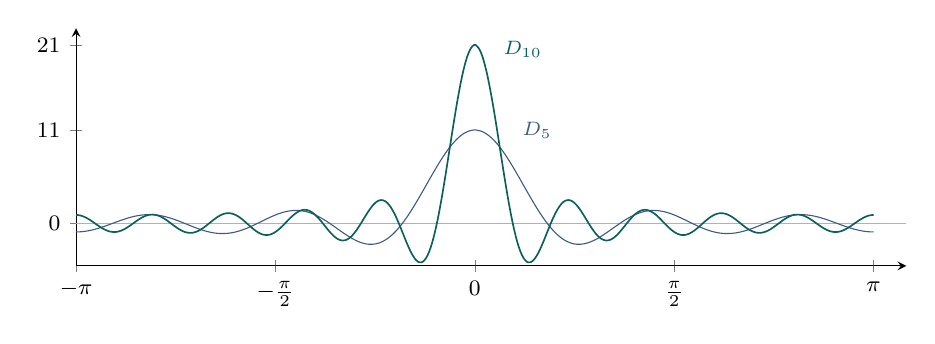
\begin{tikzpicture}
\begin{axis}[width=\textwidth,height=46mm,
  axis lines=left,xmin=-3.1416,xmax=3.4,ymin=-5,ymax=23,
  xtick={-3.1416,-1.5708,0,1.5708,3.1416},
  xticklabels={$-\pi$,$-\frac{\pi}{2}$,$0$,$\frac{\pi}{2}$,$\pi$},
  ytick={0,11,21},tick label style={font=\footnotesize},
  every axis plot/.append style={samples=500,smooth,domain=-3.1416:3.1416}]
\draw[black!30,very thin] (axis cs:-3.1416,0) -- (axis cs:3.4,0);
\addplot[thmcol,thin] {sin(deg(5.5*x))/sin(deg(x/2))};
\addplot[accent,semithick] {sin(deg(10.5*x))/sin(deg(x/2))};
\node[font=\scriptsize\sffamily,thmcol,anchor=west] at (axis cs:0.3,11) {$D_5$};
\node[font=\scriptsize\sffamily,accent,anchor=west] at (axis cs:0.15,20.5) {$D_{10}$};
\end{axis}
\end{tikzpicture}}{%
\caption{The Dirichlet kernels $D_5$ and $D_{10}$. The peak grows but the
side lobes do not die out, which is why $D_N$ is not a good averaging
kernel.}\label{fig:dirichlet}}
\end{figure}

Unfortunately $D_N$ takes negative values and its absolute integral grows like
$\log N$, so \eqref{eq:dirichlet} is not an honest average. Convergence needs
some regularity of $f$ near $x$.

\section{Pointwise convergence}

\begin{theorem}{Dirichlet}{dirichlet}
Let $f$ be $2\pi$-periodic and piecewise $C^1$. Then for every $x$,
\[
  \lim_{N\to\infty} S_N f(x) = \frac{f(x^+)+f(x^-)}{2}.
\]
In particular $S_N f(x)\to f(x)$ wherever $f$ is continuous.
\end{theorem}

\begin{proof}
Write $S_N f(x) - f(x^+)$ as an integral of $D_N$ against
$g(t)=\bigl(f(x-t)-f(x^+)\bigr)/\sin(t/2)$ over $(-\pi,0)$, and similarly for
$f(x^-)$. Piecewise smoothness makes $g$ bounded near $t=0$, and the
Riemann--Lebesgue lemma sends both integrals to zero.
\end{proof}

For the square wave this predicts $S_N f(0)\to 0$, the midpoint of the jump,
which agrees with every partial sum in Figure~\ref{fig:square}.\margintext[-2\baselineskip]{Note
the difference from the Gibbs overshoot: the
\emph{value} at each fixed $x$ converges, but the \emph{maximum} near the jump
does not. Convergence is pointwise, not uniform.}

\section{Parseval's identity}

The orthogonality relations make the coefficients behave like coordinates in an
orthonormal basis. The analogue of Pythagoras' theorem holds with infinitely
many terms.

\begin{theorem}{Parseval}{parseval}
If $f$ is square integrable on $[-\pi,\pi]$, then
\[
  \frac{1}{\pi}\int_{-\pi}^{\pi}|f(x)|^2\,dx
  = \frac{a_0^2}{2} + \sum_{n=1}^{\infty}\bigl(a_n^2+b_n^2\bigr).
\]
\end{theorem}

\begin{keyidea}
Energy is conserved between the two descriptions of $f$: the mean square of
the function equals the sum of the squares of its coefficients.
\end{keyidea}

\begin{example}{The Basel problem}{basel}
Use Parseval's identity for $f(x)=x$ to evaluate $\sum_{n\ge1}1/n^2$.
\begin{solution}
From Table~\ref{tab:series}, $a_n=0$ and $b_n = 2(-1)^{n+1}/n$. The left side is
$\frac{1}{\pi}\int_{-\pi}^{\pi}x^2\,dx = \frac{2\pi^2}{3}$. Parseval gives
\[
  \frac{2\pi^2}{3} = \sum_{n=1}^{\infty}\frac{4}{n^2}
  \qquad\Longrightarrow\qquad
  \sum_{n=1}^{\infty}\frac{1}{n^2} = \frac{\pi^2}{6}.
\]
This is Euler's 1734 result, here obtained in three lines.
\end{solution}
\end{example}

\section{Back to the heat equation}

We can now finish the problem that opened Lecture~3. The temperature
$u(x,t)$ on a ring of circumference $2\pi$ satisfies $u_t = u_{xx}$ with
$u(x,0)=f(x)$. Expanding $f$ as in \eqref{eq:fs} and evolving each mode
separately,
\begin{align*}
  u(x,t) &= \frac{a_0}{2} + \sum_{n=1}^{\infty} e^{-n^2 t}
            \bigl(a_n\cos nx + b_n\sin nx\bigr).
\end{align*}
The factor $e^{-n^2t}$ damps high frequencies fastest, so for every $t>0$ the
coefficients decay faster than any power of $n$ and $u$ is smooth, even when
$f$ is the square wave.\sidenote{This instant smoothing is special to
diffusion. The wave equation, in Lecture~6, keeps jumps forever.}

\begin{example}{Cooling a half-heated ring}{ring}
The ring starts with temperature $1$ on $(0,\pi)$ and $-1$ on $(-\pi,0)$.
How quickly does it approach equilibrium?
\begin{solution}
By Example~\ref{ex:square} only odd sine modes are present, so
\[
  u(x,t) = \frac{4}{\pi}\sum_{n\ \mathrm{odd}}\frac{e^{-n^2t}}{n}\sin nx .
\]
For $t\ge 1$ the first term dominates, since the next one is smaller by a
factor $\tfrac13 e^{-8t}\le\tfrac13 e^{-8}\approx 1.1\times10^{-4}$. The ring therefore relaxes to the mean
temperature $0$ like $\frac{4}{\pi}e^{-t}\sin x$: one smooth bump that
fades at unit rate.
\end{solution}
\end{example}

\section{Exercises}

\begin{exercise}{}{parsevalx2}
Apply Parseval's identity to $f(x)=x^2$ and deduce that
$\sum_{n\ge1}1/n^4 = \pi^4/90$.
\end{exercise}

\begin{exercise}{Uniform convergence}{uniform}
Show that if $f$ is continuous, $2\pi$-periodic and piecewise $C^1$, then
$\sum_n(|a_n|+|b_n|)<\infty$. Conclude that $S_Nf\to f$ uniformly. Which
hypothesis fails for the square wave?
\end{exercise}

\end{document}
